\documentclass[border=10pt]{standalone}

\usepackage{tikz}
\usepackage{tikzsymbols}
\usetikzlibrary{calc,patterns,shapes.geometric}

\def\centerarc[#1](#2)(#3:#4:#5){\draw[#1] ($(#2)+({#5*cos(#3)},{#5*sin(#3)})$) arc (#3:#4:#5);}

\begin{document}
	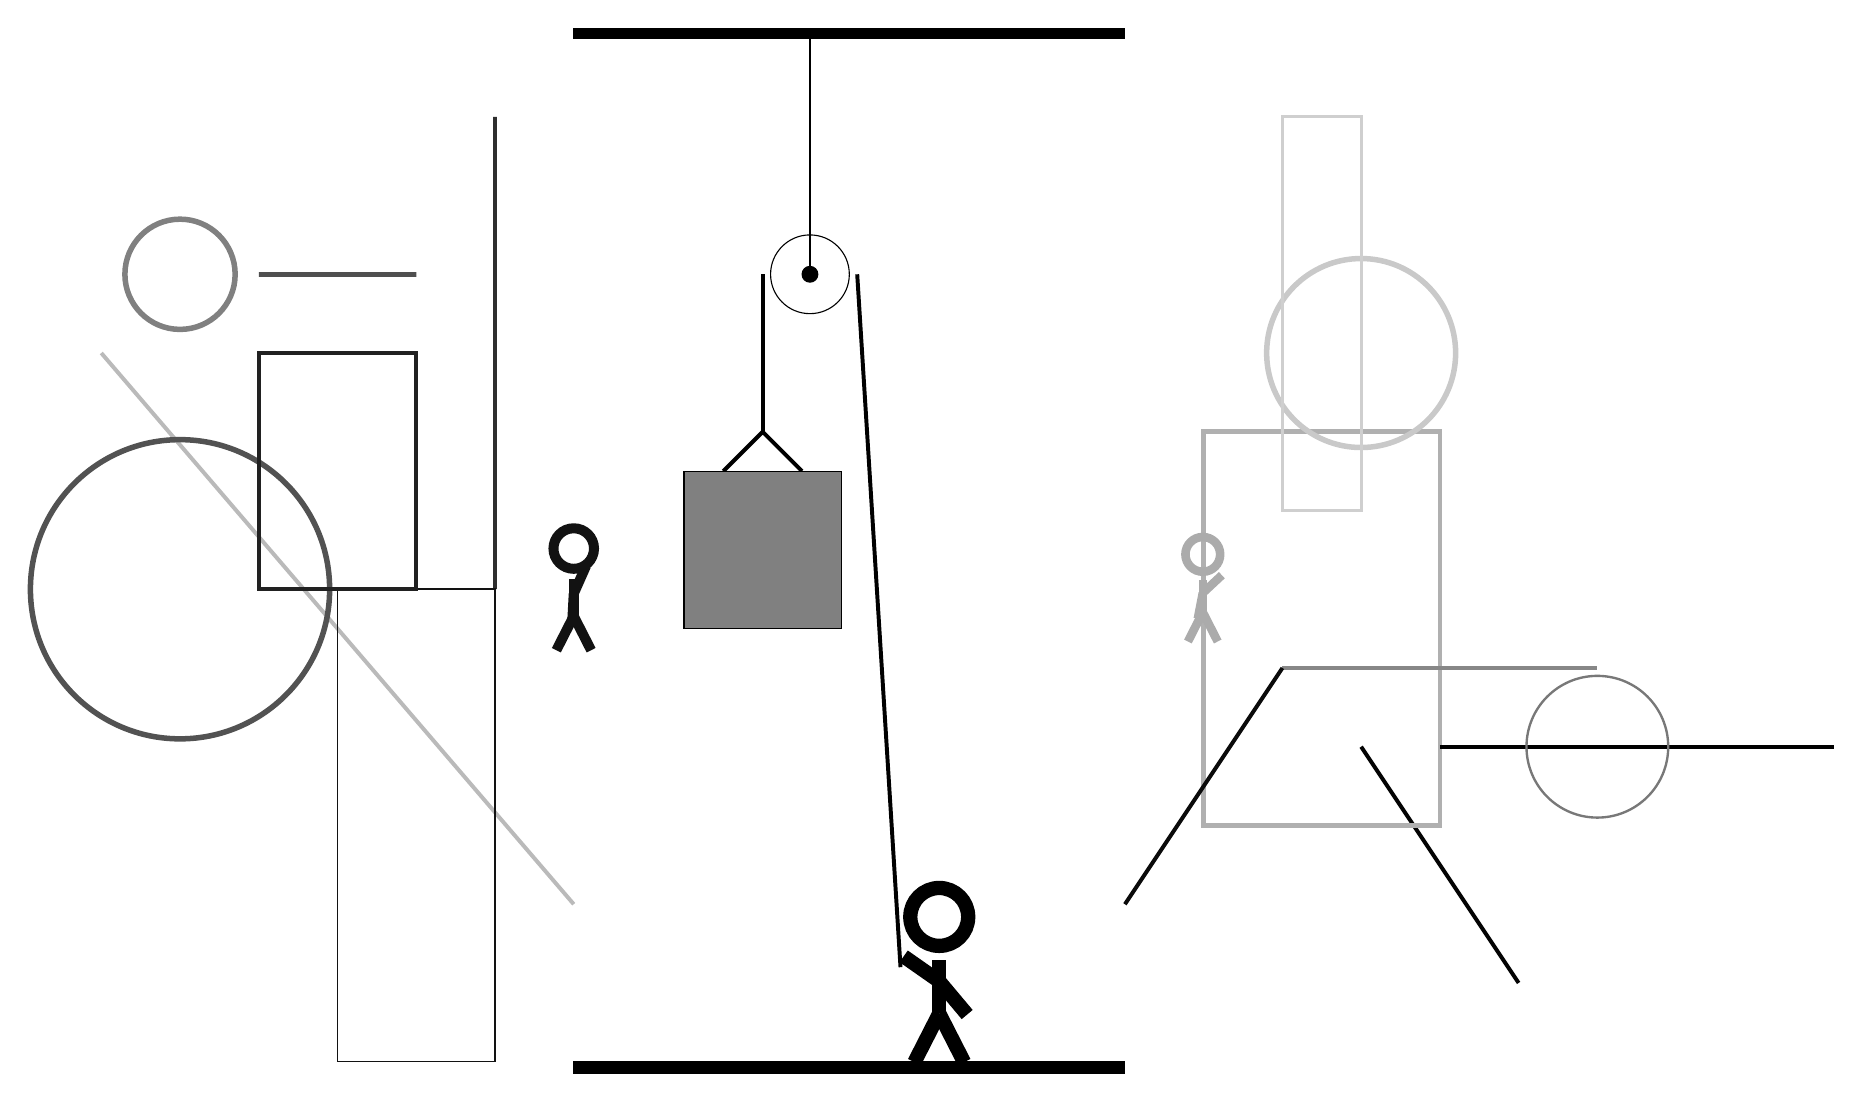
\begin{tikzpicture}
		%%%%% START %%%%%
		
		\draw[fill=black] (-2, 10) rectangle (5, 10.125);
		
		\draw (1, 7) circle (0.5);
		\draw[fill=black] (1, 7) circle (0.1);
		\draw (1, 10) -- (1, 7);
		
		\node[line width=0.4mm, color=black!93] at (-2, 3) {\Strichmaxerl[7][87][66]};
		
		\draw[line width=0.6mm, color=black!82] (-3, 9) rectangle (-3, 3);
		\draw[line width=0.5mm, color=black!99](8, 1) -- (10, -2);
		\draw[line width=0.5mm, color=black!27](-2, -1) -- (-8, 6);
		
		\draw[line width=0.6mm, color=black!31] (6, 5) rectangle (9, 0);
		
		\draw [line width=0.7mm, color=black!68](-7, 3) circle (1.9);
		\draw[line width=0.2mm, color=black!93] (-3, -3) rectangle (-5, 3);
		
		\draw [line width=0.7mm, color=black!21](8, 6) circle (1.2);
		\draw[line width=0.5mm, color=black!100](9, 1) -- (14, 1);
		
		\draw[line width=0.5mm, color=black!47](7, 2) -- (11, 2);
		\draw [line width=0.7mm, color=black!50](-7, 7) circle (0.7);
		\draw [line width=0.3mm, color=black!53](11, 1) circle (0.9);
		\draw[line width=0.7mm, color=black!69] (-4, 7) rectangle (-6, 7);
		
		\draw[line width=0.4mm, color=black!19] (7, 9) rectangle (8, 4);
		\draw[line width=0.5mm, color=black!96](5, -1) -- (7, 2);
		\draw[line width=0.5mm, color=black!87] (-4, 3) rectangle (-6, 6);
		\node[line width=0.6mm, color=black!33] at (6, 3) {\Strichmaxerl[6][79][43]};
		
		\draw[line width=0.5mm] (-0.1, 4.5) -- (0.4, 5.0) -- (0.9, 4.5);
		\draw[fill=black!50] (-0.6, 4.5) rectangle (1.4, 2.5);
		
		\draw[line width=0.5mm] (0.4, 7) -- (0.4, 5.0);
		\centerarc[line width=0.5mm](1, 7)(0:180:0.6);
		\draw[line width=0.5mm](1.6, 7) -- (2.15, -1.8);
		
		\node at (2.6, -1.9) {\Strichmaxerl[10][-35][-50]};
		
		\draw[fill=black] (-2, -3) rectangle (5, -3.15);
		
		%%%%% END %%%%%
	\end{tikzpicture}
\end{document}